\documentclass[a4paper,14pt]{article}
\usepackage{float}
\usepackage{extsizes}
\usepackage{amsmath}
\usepackage{amssymb}
\everymath{\displaystyle}
\usepackage{geometry}
\usepackage{fancyhdr}
\usepackage{multicol}
\usepackage{graphicx}
\usepackage[brazil]{babel}
\usepackage[shortlabels]{enumitem}
\usepackage{cancel}
\usepackage{textcomp}
\columnsep=2cm
\hoffset=0cm
\textwidth=8cm
\setlength{\columnseprule}{.1pt}
\setlength{\columnsep}{2cm}
\renewcommand{\headrulewidth}{0pt}
\geometry{top=1in, bottom=1in, left=0.7in, right=0.5in}

\pagestyle{fancy}
\fancyhf{}
\fancyfoot[C]{\thepage}

\begin{document}
	
	\noindent\textbf{Matemática} 
	
	\begin{center}Operações com números inteiros, expressões numéricas e problemas \\ (Versão estudante)
	\end{center}
	
	\noindent\textbf{Nome:} \underline{\hspace{10cm}}
	\noindent\textbf{Data:} \underline{\hspace{4cm}}
	
	%\section*{Questões de Matemática}
	
	
    \begin{multicols}{2}
		\begin{enumerate}
			\item Carlos realizou o controle financeiro mensal da sua loja de esfiha pelo período de seis meses e o registrou em um gráfico.
			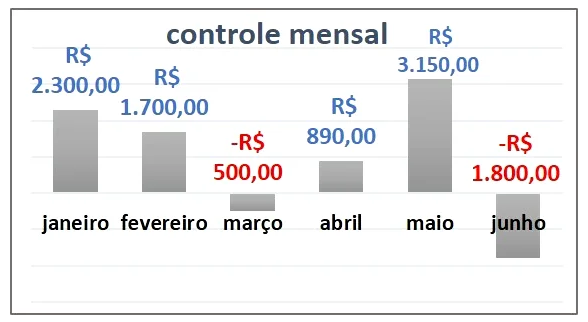
\includegraphics[width=1\linewidth]{Leonardo_imagens/imagem1}
			a) Segundo o gráfico, qual o resultado do primeiro trimestre?\\\\\\\\\\
			
			b) Qual a diferença entre o melhor e o pior resultado do semestre?\\\\\\\\\\
			
			c) Qual foi o saldo semestral?\\\\\\\\\\\\\\
			
			\newpage
			
			\item Situação Problema \\\\
			Patrícia é proprietária de uma loja de rações para cães e gatos. Este mês ela adquiriu 400 kg de ração para cachorros a um custo de R\$ 12,00 o quilograma e, 100 kg de ração para gatos ao custo de R\$ 7,50 o quilograma. Considerando que o preço de venda da ração para cachorro é de R\$ 22,00 e para gatos R\$ 19,50 e que até o momento ela vendeu 143 kg de ração de cachorro e 86 kg de ração para gatos, em relação ao investimento inicial, ela já obteve lucro ou ainda não cobriu o custo? \\
			
			Represente a situação com operações e represente utilizando números inteiros. \\
			
			\newpage
			
			\item Efetue as operações com números inteiros:
			\begin{enumerate}[a)]
				\item $-123 + 235 + 899 =$ \\\\\\\\\\\\\\
				\item $(-21)-(+81)-(-50) =$  \\\\\\\\\\\\\\
				\item $(-19)(+30)(-2) = $  \\\\\\\\\\\\\\
				\item $(+90):(-30) = $  \\\\\\\\\\\\\\
				\item $(3^2 + 6^3) = $  \\\\\\\\\\
				\item $5(10^2 + 11^2) = $  \\\\\\\\\\\\\\
				\item $(20 + 10 -((15):(+5))) = $  \\\\\\\\\\\\\\
				\item $(-5)(+3)-(9)^5 = $  \\\\\\\\\\\\\\
				\item $(-1)^{100} \cdot (-1)^{101} -(1)^0 = $  \\\\\\\\\\\\\\
				\item $(90)^0 + 155 + 1590^0 - 3 = $  
			\end{enumerate}
        \end{enumerate}
    $~$ \\ $~$ \\ $~$ \\ $~$ \\ $~$ \\ $~$ \\ $~$
    \end{multicols}
\end{document}